\section{Experimental Results}

This section presents the experimental evaluation of the 12 search strategies described in Section~\ref{sec:adaptive}, comparing their performance across instances of varying complexity.

\subsection{Experimental Setup}

The benchmarks were executed under the following conditions:

\begin{itemize}
    \item \textbf{Solver:} Gecode via MiniZinc 2.x
    \item \textbf{Timeout:} 300 seconds per instance (as specified by the project requirements)
    \item \textbf{Instances:} 60 random permutations organized as follows:
    \begin{itemize}
        \item Vector sizes: $N \in \{5, 10, 15, 20, 25, 30\}$
        \item 10 different permutations for each size
    \end{itemize}
    \item \textbf{Strategies tested:} 12 (see Table~\ref{tab:strategies})
    \item \textbf{Total executions:} $60 \times 12 = 720$
\end{itemize}

\subsection{Reliability Analysis}

Figure~\ref{fig:success} shows the number of instances solved (out of 10) for each strategy at different vector sizes.

\begin{figure}[H]
    \centering
    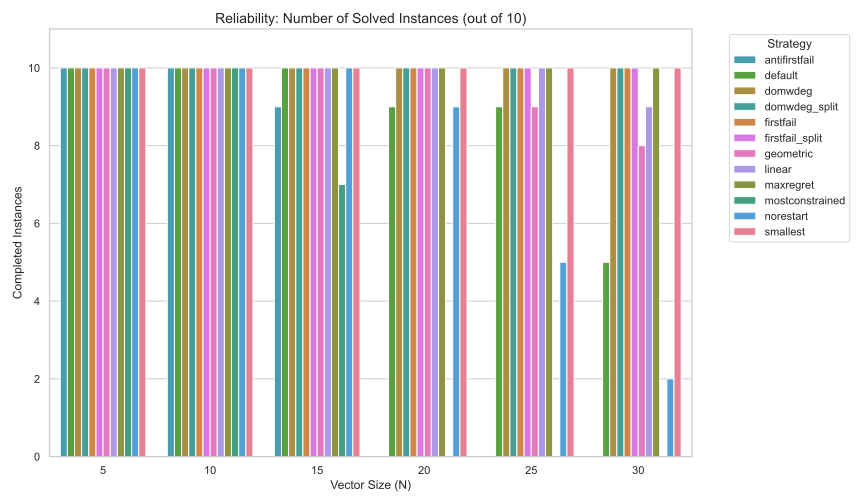
\includegraphics[width=0.95\textwidth]{img/02_successo_vs_n.pdf}
    \caption{Number of solved instances per strategy and vector size. All strategies achieve 100\% success for small instances ($N \leq 10$), but significant differences emerge for larger problems.}
    \label{fig:success}
\end{figure}

The success rate heatmap (Figure~\ref{fig:heatmap_success}) provides a clearer view of strategy reliability.

\begin{figure}[H]
    \centering
    \includegraphics[width=0.85\textwidth]{img/05_heatmap_successo.pdf}
    \caption{Success rate (\%) by strategy and vector size. Green indicates 100\% success, red indicates complete failure (0\%).}
    \label{fig:heatmap_success}
\end{figure}

Six strategies maintain perfect reliability (100\% success rate) across all instance sizes: \texttt{smallest}, \texttt{firstfail}, \texttt{firstfail\_split}, \texttt{domwdeg}, \texttt{domwdeg\_split}, and \texttt{maxregret}. These strategies prove robust even for the most challenging instances with $N = 30$.

On the opposite end, the \texttt{mostconstrained} and \texttt{antifirstfail} strategies fail completely for $N \geq 20$, reaching timeout on all instances. This suggests that these variable selection heuristics are fundamentally unsuitable for our problem structure.

The \texttt{norestart} strategy shows progressive degradation, dropping from 100\% success ($N \leq 15$) to just 20\% at $N = 30$. This confirms the critical importance of restart policies for avoiding search stagnation in larger instances.

Finally, the default Gecode configuration maintains reasonable performance for medium-sized instances but drops to 50\% success rate at $N = 30$, indicating that customized search strategies can significantly outperform the solver's default behavior.

\subsection{Performance Analysis}

Figure~\ref{fig:heatmap_time} presents the average solving time for each strategy-size combination.

\begin{figure}[H]
    \centering
    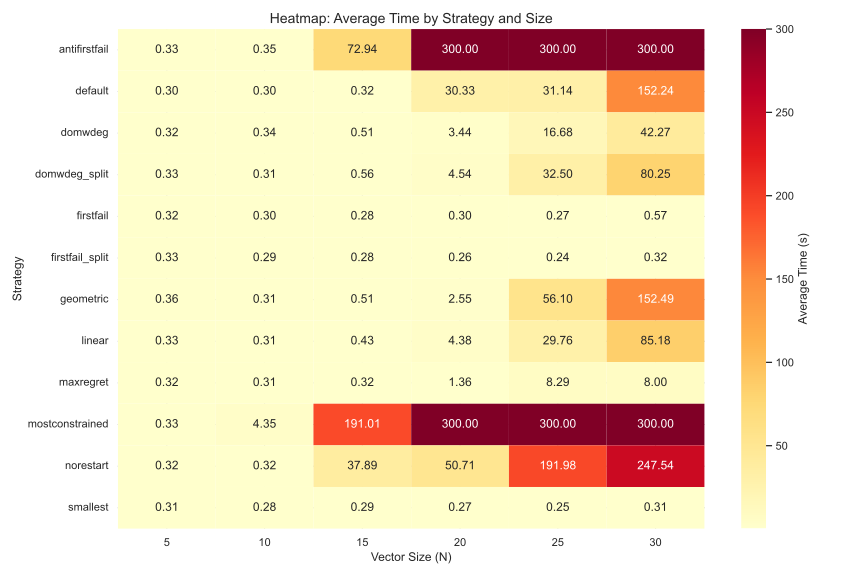
\includegraphics[width=0.85\textwidth]{img/04_heatmap_tempo.pdf}
    \caption{Average solving time (seconds) by strategy and vector size. Darker colors indicate longer times; values of 300s represent timeout.}
    \label{fig:heatmap_time}
\end{figure}


The \texttt{smallest}, \texttt{firstfail}, and \texttt{firstfail\_split} strategies consistently achieve sub-second solving times across all instance sizes, with times ranging from 0.31s to 0.57s even for $N = 30$. These strategies demonstrate excellent scalability.

In contrast, strategies like \texttt{geometric}, \texttt{linear}, and \texttt{domwdeg\_split} show significant time increases for larger instances, reaching 80--150 seconds at $N = 30$. This suggests that certain restart policies and value selection heuristics introduce overhead that becomes problematic as problem size grows.

The \texttt{mostconstrained} strategy already struggles at $N = 15$ with an average time of 191 seconds, and times out completely for $N \geq 20$. This is a particularly important finding, as the ``most constrained'' heuristic is often considered a reasonable default choice.

Comparing \texttt{norestart} with other strategies clearly demonstrates the benefit of restart mechanisms: without restarts, solving time explodes from 0.32s at $N = 5$ to 247.54s at $N = 30$. This three-orders-of-magnitude increase underscores how easily the solver can get trapped in unproductive search regions.

\subsection{Strategy Ranking}

Figure~\ref{fig:ranking} presents the overall ranking of strategies based on average solving time (computed only on successfully solved instances).

\begin{figure}[H]
    \centering
    \includegraphics[width=0.85\textwidth]{img/06_ranking_strategie.pdf}
    \caption{Strategy ranking by average solving time. Lower times indicate better performance.}
    \label{fig:ranking}
\end{figure}

The ranking reveals three distinct performance tiers. The \textbf{top tier} (under 1 second average) includes \texttt{smallest} (0.283s), \texttt{firstfail\_split} (0.286s), \texttt{firstfail} (0.339s), and \texttt{default} (0.875s). These strategies are suitable for real-time applications where response time is critical.

The \textbf{middle tier} (1-15 seconds average) comprises \texttt{maxregret} (3.1s), \texttt{domwdeg} (10.6s), \texttt{antifirstfail} (15.0s), and \texttt{linear} (15.3s). While slower, these strategies still complete within reasonable time bounds for most applications.

The \textbf{bottom tier} (over 15 seconds average) includes \texttt{domwdeg\_split} (19.7s), \texttt{geometric} (21.5s), \texttt{norestart} (23.6s), and \texttt{mostconstrained} (39.1s). These strategies are not recommended for production use, as their performance degrades significantly with problem size.

\subsection{Discussion}

The experimental results lead to several important conclusions regarding search strategy design for the sorting problem.

\paragraph{Variable selection is crucial.} The \texttt{smallest} heuristic, which selects the move variable with the smallest current domain, proves to be the most effective choice. This is intuitive for our problem: moves with smaller domains are closer to being fixed and represent more constrained decisions. By committing to these variables first, the solver quickly narrows the search space.

\paragraph{The first-fail principle works.} Both \texttt{firstfail} and \texttt{firstfail\_split} confirm the effectiveness of the first-fail principle for this problem. Prioritizing variables with smaller domains leads to earlier detection of dead ends, allowing the solver to backtrack sooner and avoid exploring fruitless subtrees.

\paragraph{Restarts are essential.} The dramatic performance difference between strategies with and without restarts demonstrates that restart mechanisms are critical for avoiding search stagnation. The \texttt{norestart} strategy's 80\% failure rate at $N = 30$ versus 100\% success for strategies with Luby restarts provides compelling evidence for this conclusion.

\paragraph{Domain-weighted degree has mixed results.} While \texttt{domwdeg} maintains a 100\% success rate, its average time is significantly higher than simpler heuristics like \texttt{firstfail}. The learning overhead of tracking constraint weights may not pay off for instances of this size, where simpler static heuristics suffice.

\paragraph{Anti-first-fail fails.} The \texttt{antifirstfail} strategy, which prioritizes variables with larger domains, performs poorly as expected. This confirms that our problem benefits from early commitment to constrained choices rather than deferring difficult decisions.

\paragraph{Most-constrained is misleading.} Despite its name, the \texttt{mostconstrained} heuristic (selecting the variable involved in the most constraints) fails completely for larger instances. This suggests that constraint count is not a good proxy for variable importance in our model, where all move variables participate in similar constraint structures.

\subsection{Future Work}

A natural direction for future work is to compare the constraint programming approach not only in terms of execution time, but also in terms of memory accesses and the number of swaps performed, with respect to classical sorting algorithms such as quicksort, mergesort, or bubble sort. This would provide a more meaningful comparison of the computational effort required by different paradigms, especially since classical algorithms are highly optimized for time but may differ in the number of elementary operations.

Another interesting extension would be to experiment with new constraints or to adapt the model to handle vectors with arbitrary values, not just permutations of $1$ to $N$. This would allow the approach to be applied to a wider range of sorting problems, including those with repeated or missing values, and could require the development of new constraint formulations or search strategies.
